\documentclass[a4paper,11pt]{article}
\input{/home/tof/Documents/Cozy/latex-include/preambule_lua.tex}
\newcommand{\showprof}{show them}  % comment this line if you don't want to see todo environment
\fancyhead[L]{Arbre - sortir du labyrinthe}
\newdate{madate}{10}{09}{2020}
%\fancyhead[R]{\displaydate{madate}} %\today
%\fancyhead[R]{Seconde - SNT}
%\fancyhead[R]{Première - NSI}
\fancyhead[R]{Terminale - NSI}
\fancyfoot[L]{~\\Christophe Viroulaud}
\AtEndDocument{\label{lastpage}}
\fancyfoot[C]{\textbf{Page \thepage/\pageref{lastpage}}}
\fancyfoot[R]{\includegraphics[width=2cm,align=t]{/home/tof/Documents/Cozy/latex-include/cc.png}}
\usepackage{tikz}

\begin{document}
\begin{Form}
\begin{commentprof}
arbre-labyrinthe.zip sur site
\end{commentprof}
\section{Problématique}
Les chemins d'un labyrinthe peuvent être représentés par un graphe. Dans le cas d'un labyrinthe sans boucle ni case inaccessible ce graphe est un arbre.
\begin{center}
\shadowbox{\parbox{12cm}{\centering Comment retrouver la sortie d'un labyrinthe à l'aide d'un arbre?}}
\end{center}
\section{Visualisation du problème}
Pour représenter le labyrinthe (figure \ref{laby}) en mémoire on peut utiliser un graphe.
\begin{commentprof}
ici c'est un arbre car labyrinthe sans boucle ni case isolée.
\end{commentprof}
\begin{center}
\centering
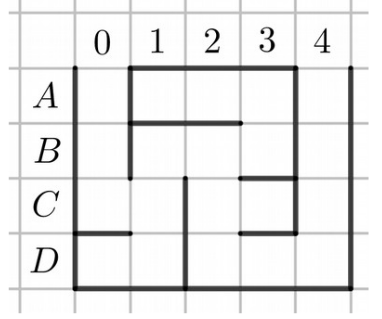
\includegraphics[width=5cm]{ressources/labyrinthe.png}
\captionof{figure}{Labyrinthe}
\label{laby}
\end{center}
\begin{activite}
\begin{enumerate}
\item Télécharger et extraire \emph{arbre-labyrinthe.zip} sur le site \url{https://cviroulaud.github.io} .
\item Créer un fichier \emph{labyrinthe.py}.
\item Construire le graphe représentatif du labyrinthe (figure \ref{laby}).
\item À l'aide d'une méthode de la classe \emph{Graphe} Donner le chemin du départ (A0) à la sortie (A4).
\item À l'aide de la bibliothèque \emph{networkx}, représenter l'arbre des chemins du labyrinthe.
\end{enumerate}
\end{activite}
\section{Labyrinthe aléatoire}
\subsection{Méthodes utiles}
\begin{activite}
\begin{enumerate}
\item Ouvrir la fichier \emph{labyrinthe-maxi.py} . Il contient la classe \emph{Labyrinthe}.
\item Compléter la méthode \textbf{creer\_sommets(self)$\;\rightarrow\;$None} qui crée les sommets du graphe.
\item Compléter la méthode \textbf{get\_voisins(self, en\_cours: object)->list:} qui renvoie une liste des nœuds voisins de \emph{en\_cours}. Cette méthode utilise le tuple \emph{delta} qui permet de repérer chaque voisin de \emph{en\_cours}.
\end{enumerate}
\end{activite}
\subsection{Construire le labyrinthe}
Le principe de construction utilise un parcours en profondeur du graphe. Les figures \ref{e1} à \ref{e6} décrivent l'algorithme.
\begin{center}
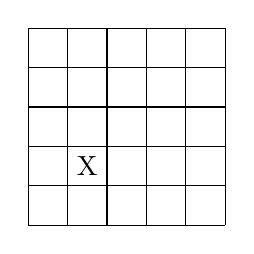
\begin{tikzpicture}[scale=0.5]
\draw (0,0) grid (5,5);
\node at(1.5,1.5) {X};
\end{tikzpicture}
\captionof{figure}{Choisir une cellule, l'empiler}
\label{e1}
\end{center}
On itère sur la pile tant qu'elle n'est pas vide.
\begin{center}
\textbf{Première itération}\medskip\\
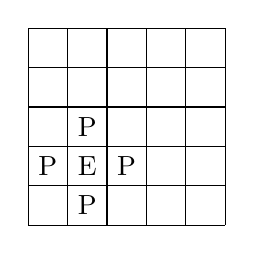
\begin{tikzpicture}[scale=0.5]
\draw (0,0) grid (5,5);
\node at(1.5,1.5) {E};
\node at(0.5,1.5) {P};
\node at(2.5,1.5) {P};
\node at(1.5,0.5) {P};
\node at(1.5,2.5) {P};
\end{tikzpicture}
\captionof{figure}{Dépiler}
\label{e2}
\end{center}
\begin{center}
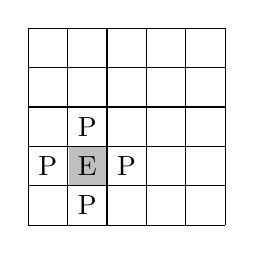
\begin{tikzpicture}[scale=0.5]
\draw (0,0) grid (5,5);
\node[fill=gray!50] at(1.5,1.5) {E};
\node at(0.5,1.5) {P};
\node at(2.5,1.5) {P};
\node at(1.5,0.5) {P};
\node at(1.5,2.5) {P};
\end{tikzpicture}
\captionof{figure}{Marquer le nœud \emph{visité} et empiler tous les voisins}
\label{e3}
\end{center}
À ce stade aucun voisin n'est encore dans le labyrinthe. Aucune arête n'est encore créée. La première itération est terminée.
\begin{center}
\textbf{Deuxième itération}\medskip\\
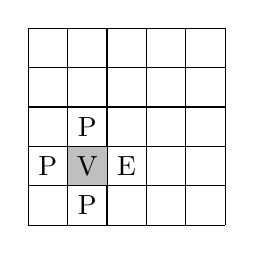
\begin{tikzpicture}[scale=0.5]
\draw (0,0) grid (5,5);
\node[fill=gray!50] at(1.5,1.5) {V};
\node at(0.5,1.5) {P};
\node at(2.5,1.5) {E};
\node at(1.5,0.5) {P};
\node at(1.5,2.5) {P};
\end{tikzpicture}
\captionof{figure}{Dépiler}
\label{e4}
\end{center}
\begin{center}
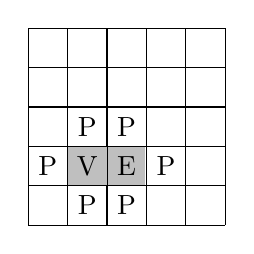
\begin{tikzpicture}[scale=0.5]
\draw (0,0) grid (5,5);
\node[fill=gray!50] at(1.5,1.5) {V};
\node at(0.5,1.5) {P};
\node[fill=gray!50] at(2.5,1.5) {E};
\node at(1.5,0.5) {P};
\node at(1.5,2.5) {P};
\node at(3.5,1.5) {P};
\node at(2.5,0.5) {P};
\node at(2.5,2.5) {P};
\end{tikzpicture}
\captionof{figure}{Le marquer \emph{visité} et empiler tous les voisins}
\label{e5}
\end{center}
\begin{center}
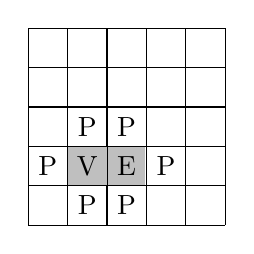
\begin{tikzpicture}[scale=0.5]
\draw (0,0) grid (5,5);
\node[fill=gray!50] at(1.5,1.5) {V};
\node at(0.5,1.5) {P};
\node[fill=gray!50] at(2.5,1.5) {E};
\node at(1.5,0.5) {P};
\node at(1.5,2.5) {P};
\node at(3.5,1.5) {P};
\node at(2.5,0.5) {P};
\node at(2.5,2.5) {P};
\end{tikzpicture}
\captionof{figure}{Créer \underline{une} arête entre le labyrinthe et le nœud en cours.}
\label{e6}
\end{center}
Pour créer cette arête il faut vérifier si un des voisins du nœud en cours est déjà dans le labyrinthe.
\begin{activite}
Compléter la méthode \textbf{creer\_dfs(self)$\;\rightarrow\;$None} .
\end{activite}
\subsection{Sortir du labyrinthe}
\begin{activite}
\begin{enumerate}
\item Exécuter la méthode \emph{affiche\_chemins}. Il faut voir le labyrinthe comme un arbre de racine (0,0).
\item Compléter la méthode \textbf{chemin\_sortie(self)$\;\rightarrow\;$list} qui renvoie le parcours entre l'entrée en haut à gauche du labyrinthe et la sortie en bas à droite.
\end{enumerate}
\end{activite}
\end{Form}
\end{document}